\chapter{Semantic Segmentation}
\label{ch:lesson42}

Classification labels a whole image. Detection (Chapters~\ref{ch:lesson40}--\ref{ch:lesson41}) labels a handful of boxes. \textbf{Semantic segmentation} goes one step further: label \emph{every pixel} with a class/category. The original deep-learning method is the \textbf{fully convolutional network (FCN)} (\citelink{long2015fcn}{Long, Shelhamer \& Darrell, 2015}), which replaces a classifier's fully-connected layers with convolutions, then upsamples the result back to the input resolution. The output is a dense, per-pixel prediction instead of a single label for the whole image. This chapter builds that idea from scratch, checks it against a real pretrained FCN, and then adds one specific enhancement to it --- skip connections.

\section{A 3-class pixel labeling task}

Create an image with several small circles and squares scattered on a background. The target is a full per-pixel class map: 0 = background, 1 = circle, 2 = square. Class pixel fractions in the training set are heavily imbalanced: background $0.866$, circle $0.046$, square $0.088$ (Figure~\ref{fig:l42-1}).

\begin{figure}[h]
\centering
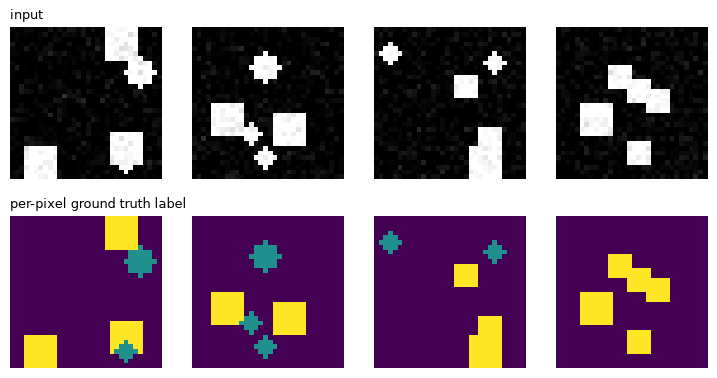
\includegraphics[width=0.9\textwidth]{figures/lesson42_fig01.png}
\caption{Input images (top row) and their per-pixel ground-truth labels (bottom row).}
\label{fig:l42-1}
\end{figure}

\section{A minimal FCN-style network}

A segmentation network outputs a class-probability vector for every pixel, so its output is the same spatial size as the input. The \textbf{encoder} is an ordinary CNN, downsampling twice via max pooling (Chapter~\ref{ch:lesson34}) to build up semantically rich features with a wide receptive field (Chapter~\ref{ch:lesson11}'s pyramid). The \textbf{decoder} then upsamples that coarse bottleneck straight back to full resolution. That's the entire FCN recipe: just downsample then upsample.

\begin{lstlisting}
class FCNTiny(nn.Module):
    def forward(self, x):
        f1 = self.enc1(x)                # (B,16,H,W)
        f2 = self.enc2(self.pool(f1))    # (B,32,H/2,W/2)
        f3 = self.enc3(self.pool(f2))    # (B,64,H/4,W/4)  -- the bottleneck
        d2 = self.dec2(self.up(f3))      # upsample only -- no fusion with f2
        d1 = self.dec1(self.up(d2))      # upsample only -- no fusion with f1
        return self.out(d1)
\end{lstlisting}

Trained for 200 epochs with cross-entropy loss: pixel accuracy $98.1\%$, per-class IoU of $0.984$ (background), $0.736$ (circle), $0.891$ (square), giving a mean IoU of $0.870$.

\section{In practice: FCN on a real photo}

\code{torchvision} ships \textbf{FCN} (\citelink{long2015fcn}{Long et al., 2015}), pretrained on COCO images (labeled with the 21 Pascal VOC categories --- 20 object classes plus background). This is architecturally the same recipe as \code{FCNTiny} above: encoder, then upsampling.

\begin{figure}[h]
\centering
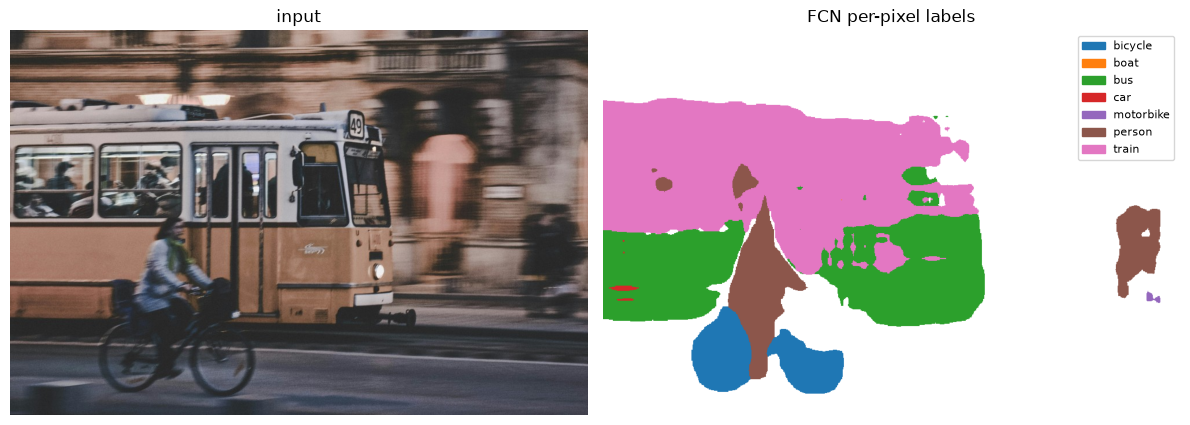
\includegraphics[width=0.95\textwidth]{figures/lesson42_fig02.png}
\caption{Real FCN per-pixel labels on a street photo. \attrib{Photo by Felix Hanspach on Unsplash.}}
\label{fig:l42-2}
\end{figure}

The cyclist is cleanly labeled \code{person}, with the bicycle's wheels correctly labeled \code{bicycle} just below --- both real, correctly-placed detections (Figure~\ref{fig:l42-2}). The tram is where it gets interesting: the model splits it between \code{train} (the upper, windowed section) and \code{bus} (the lower body) rather than picking one label for the whole vehicle. That's not really a mistake so much as an honest reflection of VOC's limited vocabulary --- a tram is a genuinely ambiguous case between ``train'' and ``bus'' for a model that was never given a ``tram'' class to choose from, and the two guesses roughly track a real visual seam in the vehicle (windows vs.\ body) rather than being random. A second, smaller \code{person} blob on the right edge catches the blurred pedestrian in the background.

\section{Adding skip connections: U-Net}

\code{FCNTiny}'s decoder only sees the pooled, upsampled bottleneck features. After two rounds of pooling, that bottleneck has just a quarter of the input's spatial resolution, and small or closely-packed shapes can blur together or lose their boundaries entirely at that resolution. \textbf{U-Net} (\citelink{ronneberger2015}{Ronneberger, Fischer \& Brox, 2015}) fixes this with \textbf{skip connections}: at each decoder stage, it concatenates the encoder's feature map from the \emph{matching resolution}, preserving the fine-grained details that would otherwise be lost during pooling. This is similar in spirit to Chapter~\ref{ch:lesson37}'s residual connections, but the purpose and mechanism differ: U-Net concatenates features across the encoder-decoder boundary, rather than adding a residual update within a single network stack.

\begin{lstlisting}
class UNetTiny(nn.Module):
    def forward(self, x):
        f1 = self.enc1(x)
        f2 = self.enc2(self.pool(f1))
        f3 = self.enc3(self.pool(f2))
        d2 = self.dec2(torch.cat([self.up(f3), f2], dim=1))    # skip from f2
        d1 = self.dec1(torch.cat([self.up(d2), f1], dim=1))    # skip from f1
        return self.out(d1)
\end{lstlisting}

Trained identically for 200 epochs:

\begin{center}
\renewcommand{\arraystretch}{1.3}
\begin{tabular}{lrr}
\hline
 & \textbf{pixel acc} & \textbf{mean IoU} \\
\hline
FCN (no skip)  & 98.1\% & 0.870 \\
U-Net (skip)   & 99.5\% & 0.943 \\
\hline
\end{tabular}
\end{center}

\begin{figure}[h]
\centering
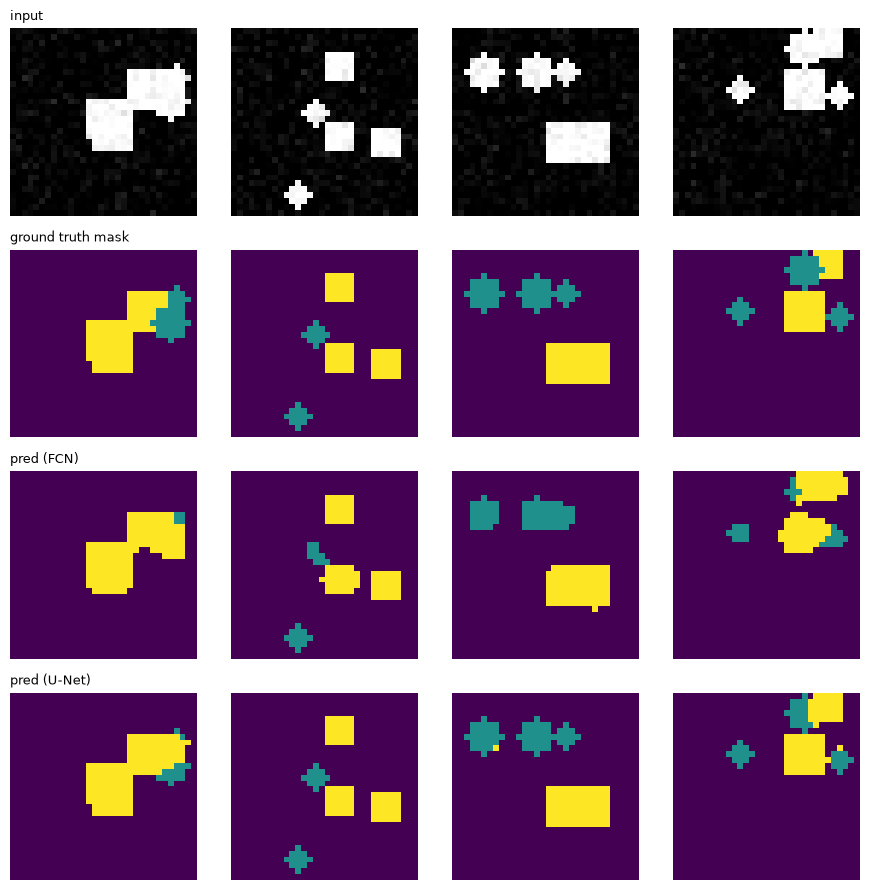
\includegraphics[width=0.9\textwidth]{figures/lesson42_fig03.png}
\caption{Input, ground truth, FCN prediction, and U-Net prediction, for four test scenes.}
\label{fig:l42-3}
\end{figure}

For small, tightly packed shapes, skip connections provide a substantial mean-IoU improvement over a plain FCN, visible directly in Figure~\ref{fig:l42-3}. An FCN cannot recover detail that was lost in the low-resolution bottleneck, because interpolation can only work on existing information. Skip connections fix this problem by giving the decoder a second, non-bottlenecked path to the encoder's high-resolution features, so precise boundaries never have to survive the bottleneck in the first place.

This helps explain why U-Net remains popular for tasks requiring precise boundaries, especially medical imaging. But skip connections are not universal: popular networks like plain FCN and DeepLabV3 have none, and even DeepLabV3+ adds only a single one, not a full U-Net-style connection at every resolution. So while skip connections are a useful tool, they are not a requirement --- their value depends on how much fine spatial detail the task demands.

\subsection*{Exercises}
\begin{enumerate}
  \item Increase \code{n\_shapes} from 5 to 10, making the scene more crowded. Does the \code{FCNTiny}-vs-\code{UNetTiny} gap in mean IoU get larger or smaller? What does that suggest about when skip connections matter most?
  \item This chapter's loss is plain per-pixel cross-entropy. Try \code{F.cross\_entropy(logits, Mt, weight=inverse\_class\_freq)} (Chapter~\ref{ch:lesson36}'s imbalance fix, applied here) to see whether it changes the circle/square IoU balance.
  \item \code{nn.Upsample(mode='nearest')} was used for simplicity. Try \code{mode='bilinear', align\_corners=False} instead (Chapter~\ref{ch:lesson09}'s bilinear interpolation, now inside a network) and compare mean IoU for both \code{FCNTiny} and \code{UNetTiny}. Does the smoother upsampling help more or less than the skip connection does?
  \item Print the confidence (softmax probability of the predicted class) at a few pixels along the seam where the real FCN result switches from \code{train} to \code{bus} on the tram. Is the model confidently split, or genuinely uncertain right at that boundary?
\end{enumerate}

\vfill
\fullcode{lesson42}{lesson42_semantic_segmentation}
